%%%%%%%%%%%%%%%%%%%%%%%%%%%%%%%%%%%%%%%%%
% University/School Laboratory Report
% LaTeX Template
% Version 3.1 (25/3/14)
%
% This template has been downloaded from:
% http://www.LaTeXTemplates.com
%
% Original author:
% Linux and Unix Users Group at Virginia Tech Wiki 
% (https://vtluug.org/wiki/Example_LaTeX_chem_lab_report)
%
% License:
% CC BY-NC-SA 3.0 (http://creativecommons.org/licenses/by-nc-sa/3.0/)
%
%%%%%%%%%%%%%%%%%%%%%%%%%%%%%%%%%%%%%%%%%


%----------------------------------------------------------------------------------------
% PACKAGES AND DOCUMENT CONFIGURATIONS
%----------------------------------------------------------------------------------------

\documentclass[letter, titlepage, 10pt]{article}

\usepackage{fancyhdr, graphicx} % Required for the inclusion of images
%\usepackage{natbib} % Required to change bibliography style to APA
\usepackage{amsmath} % Required for some math elements 

\usepackage[spanish]{babel} % Para separar correctamente las palabras
\usepackage[utf8]{inputenc} % Este paquete permite poner acentos y eñes usando c

\usepackage[titletoc,toc,title]{appendix}
\usepackage{titlepic}

\usepackage{caption}
\usepackage{subcaption}

\usepackage{color}
\usepackage[table,xcdraw]{xcolor}

\usepackage{float}
\restylefloat{table}

\definecolor{lightgrey}{rgb}{0.9,0.9,0.9}
\definecolor{darkgreen}{rgb}{0,0.6,0}

\usepackage{listings}
\lstset{language=Python,
    basicstyle=\ttfamily\bfseries,
    commentstyle=\color{red}\itshape,
  stringstyle=\color{darkgreen},
  showstringspaces=false,
  breaklines=true,  
  keywordstyle=\color{blue}
  \bfseries}


\setlength\parindent{0pt} % Removes all indentation from paragraphs

\renewcommand{\labelenumi}{\alph{enumi}.} % Make numbering in the enumerate environment by letter rather than number (e.g. section 6)
\newcommand{\abs}[1]{\left\vert#1\right\vert}
%\usepackage{times} % Uncomment to use the Times New Roman font

%----------------------------------------------------------------------------------------
% DOCUMENT INFORMATION
%----------------------------------------------------------------------------------------

\textheight=21cm
\textwidth=16.5cm   
\topmargin=-0.5cm
\oddsidemargin=0cm
\parindent=0mm


%--------------------------------------------------------------------------
\title{TALLER I \\ La Aventura de Teseo \\ Resolución de Problemas Basados en Búsqueda} % Title
\author{Brian Keith\\
  \small briankeithn@gmail.com\\
\and
  Exequiel Fuentes\\
  \small efulet@gmail.com\\
}

\titlepic{
\includegraphics[bb=0 0 242 246,scale=0.2,keepaspectratio=true]{./images/ucn_logo.jpg}}
% ucn_logo.jpg: 2017x2053 pixel, 600dpi, 8.54x8.69 cm, bb=0 0 242 246



%\renewcommand{\headrulewidth}{0pt}
%\fancyhead[L]{
\includegraphics[width=5em]{images/logo_c_ucn_small}\hspace{0.3cm}\parbox[b][4em][t]{0.8\textwidth}{Universidad Católica del Norte \\ Departamento de Ingeniería de Sistemas y Computación \\ Magíster en Ingeniería Informática}}
%\fancyhead[R]{}

%\titlehead{\centering\includegraphics[width=6cm]{placeholder}}

\date{\today}
%\publishers{blah}

%\author{Juan  \textsc{Bekios}} % Author name

%\date{\today} % Date for the report

\begin{document}

\maketitle % Insert the title, author and date
%\thispagestyle{fancy}

%\begin{center}
%\begin{tabular}{l r}
%Fecha de Entrega: &  20 de Mayo, 2014 \\ % Date the experiment was performed
%Autor: & Brian Keith \\ & Exequiel Fuentes \\
%Asignatura: & Sistemas Inteligentes\\ % Asignatura
%Profesor: & Juan Bekios-Calfa % Instructor/supervisor
%\end{tabular}
%\end{center}

% If you wish to include an abstract, uncomment the lines below
% \begin{abstract}
% Abstract text
% \end{abstract}

%----------------------------------------------------------------------------------------
% SECTION 1
%----------------------------------------------------------------------------------------

\section{Introducción}
El objetivo del presente trabajo es mostrar el desarrollo del problema del laberinto con Teseo y el Minotauro, utilizando diferentes algoritmos de búsqueda vistos en clases. Se desarrollarán los algoritmos de búsqueda en anchura, profundidad, costo uniforme y A* en Python. 

De manera formal se define la búsqueda como el proceso de examinar diferentes posibles secuencias de acciones que llevan a estados conocidos, y luego escoger la mejor secuencia. Un algoritmo de búsqueda toma un problema como su entrada y retorna una solución en la forma de una secuencia de acciones.

Los algoritmos implementados en este taller encuentran una solución al problema, para el caso de búsqueda en profundidad el camino encontrado puede no ser óptimo, pero para todos los demás se encuentra garantizado que la solución sea óptima. Se utilizó además la librería GASP de Python para mostrar el funcionamiento de los algoritmos gráficamente.

\subsection{Contexto del problema}
El problema propuesto consiste en ayudar a Teseo a encontrar la ruta más corta hacía el minotauro en el laberinto que construyó Dédalo. Una vez encontrado el minotauro, Teseo debe matarle y luego salir por la misma ruta por la que entró. Teseo dispone de la ayuda de Ariadna, una de las hijas del rey Minos, quien le ha enseñado como asesinar a la gran bestia, además, Teseo dispone de un ovillo mágico que le permite guiarse a través del laberinto, marcando la ruta que ha tomado. 

Se debe modelar el enunciado propuesto como un \textbf{problema de búsqueda} y debe resolverse utilizando los distintos algoritmos vistos en clase. Se pretende con esta experiencia comparar el rendimiento de las diferentes estrategias de búsqueda en el problema de Teseo y el minotauro.

\subsection{Experiencias Relacionadas}
Existe una gran cantidad de material referente al tema de búsqueda en internet, los problemas clásicos presentados corresponden a las N-reinas, el puzzle 8 (y sus extensiones), y por supuesto, el laberinto.

Se han encontrado varias experiencias similares al problema del laberinto. Los algoritmos de búsqueda de camino o ``pathfinding'' se utilizan mucho en la programación de vídeo juegos (A* es el algoritmo que se utiliza generalmente para esto). Uno de los problemas similares encontrados consiste en dotar a los fantasmas del juego ``Pacman'' de una rutina de búsqueda basada en el algoritmo A* para encontrar la mejor ruta con la que atacar al jugador. También se debe mencionar el artículo sobre búsqueda de caminos en laberintos de estructura desconocida, donde se hace uso de diferentes algoritmos de búsqueda no informada para encontrar la solución.

Se han encontrado también numerosas soluciones del problema de búsqueda de caminos en laberintos (las cuáles se encuentran referenciadas en la bibliografía). La implementación del taller se ha hecho en base de las soluciones encontradas en la web y del código visto en clases. Se ha utilizado programación orientada a objetos para el desarrollo del taller. Una de las soluciones encontradas utilizaba orientación a objetos, sin embargo, la lógica no se encontraba separada de la presentación. Se han mejorado las soluciones encontradas ya que se ha separado la lógica de la presentación. 

\subsection{Agentes Inteligentes}

Se han implementado dos tipos de agentes inteligentes en este taller:
\begin{itemize}
  \item{\textbf{Agente basado en objetivos: }} Este tipo de agentes realizan búsquedas sin ninguna información extra, es decir, la búsqueda es ciega, debido a esto en el peor caso deben realizar una búsqueda completa del espacio de estados. Se implementaron dos algoritmos siguiendo este enfoque (anchura y profundidad).
  \item{\textbf{Agente basado en utilidad: }}  Este tipo de agentes utilizan una métrica para buscar la solución, en este caso se usará el costo que tiene cada camino. Es importante en este tipo de agentes la definición de las funciones para evaluar los costos. Se implementaron dos algoritmos siguiendo este enfoque (costo uniforme y A*).
\end{itemize}

\subsubsection{Percepciones}
El agente recibirá como percepciones su posición actual, las posibles posiciones a donde puede moverse y además sabe la posición del minotauro. 

\subsubsection{Acciones}
Las acciones que puede realizar el agente son movimientos, puede moverse en las cuatro direcciones básicas (arriba, abajo, izquierda y derecha), a no ser que exista una muralla que se lo impida.

\subsubsection{Objetivos}
El objetivo del agente es recorrer el laberinto para encontrar al minotauro y obtener el camino más corto desde la entrada hasta él. Una vez encontrado el minotauro debe encontrar el camino más corto para la salida, sin embargo, como para esta versión del problema, la salida corresponde a la misma entrada, se debe utilizar el mismo camino original.

\subsubsection{Ambiente}
Se describe a continuación el ambiente, para ello se responde las siguientes preguntas:

\begin{itemize}
%Fuente http://www.cs.stir.ac.uk/courses/31YE/lectures/2%20-%20Environments.pdf
\item ¿El agente puede determinar inequívocamente el estado del entorno?\\
Si bien el agente no puede percibir todo el laberinto desde su posición actual, las percepciones le entregan la información necesaria y suficiente para tomar las decisiones correctas, por lo tanto el ambiente es \textbf{accesible}.

\item ¿Las acciones del agente en un estado actual determinan completamente el estado resultante?\\
Sí, las acciones que realiza el agente determinan por completo el siguiente estado, no existen elementos estocásticos y aleatorios en este ambiente, por lo tanto, el ambiente es \textbf{determinístico}.

\item ¿El estado del entorno puede cambiar mientras que el agente delibera?\\ El entorno no cambia mientras el agente delibera su siguiente movimiento, pues tanto la posición del minotauro como la estructura del laberinto se preservan a lo largo del tiempo, por lo tanto el ambiente es \textbf{estático}. (Diferente sería el problema si es que el minotauro se moviese a lo largo del laberinto en busca de Teseo)

\item ¿Los conjuntos de posibles percepciones y/o acciones son discretas?\\
Los posibles estados del ambiente, al igual que las posibles acciones que puede tomar el agente, forman un conjunto discreto. Por lo tanto el ambiente es \textbf{discreto}.

\item ¿Las acciones que toma el agente en un momento afectan las futuras acciones de este?\\
Sí, cada acción que toma el agente determina las futuras acciones que podrá tomar el agente, es decir, el agente no actúa en episodios independientes de acción cada vez que delibera, por lo tanto, el ambiente es \textbf{secuencial} (no episódico).

\item ¿Cuántos agentes actúan en el ambiente?\\
Se tiene un único agente actuando en el ambiente, por lo tanto, el ambiente es de \textbf{un sólo agente}.
\end{itemize}

\newpage

\section{Diseño de un Agente}

\subsection{Definición formal del problema}
Se definirá primero formalmente el problema de búsqueda de camino en el laberinto será definido de la siguiente forma:

\begin{itemize}
\item Se define un tablero inicial $M$ de dimensiones $MxN$ que representa un laberinto con murallas y caminos en sus posiciones.
\item Se tiene un estado inicial único $S = (x_0, y_0)$.
\item Se tiene un estados final único $F = (x_f, y_f)$ (podría ser posible definir el problema con varios estados finales).
\item Desde la posición inicial se debe llegar a la posición final realizando solo movimientos del tipo: Arriba, Abajo, Derecha e Izquierda.
\item Existe la posibilidad que no haya solución.
\item El objetivo del problema es encontrar un camino de solución óptimo.
\end{itemize}


\begin{description}
  \item[Representación del Laberinto] \hfill \\
  Antes de diseñar el agente propiamente tal, se debe definir una representación para el ambiente. El laberinto es un tablero que se representa mediante una matriz $M$ de dimensiones $N \times M$. Cada entrada $(x,y)$ de la matriz representa una posición en el tablero de laberinto. En cada posición del laberinto se puede tener uno de los siguientes elementos:
    \begin{itemize}
          \item Un ``0'' si es que la posición tiene una muralla.
          \item Un ``1'' si es que la posición está libre y se puede caminar por ella.
          \item Un ``2'' si es que la posición corresponde a la posición inicial de Teseo.
          \item Un ``3'' si es que la posición corresponde a la posición del Minotauro.
          \item Un ``4'' si es que la posición ya ha sido recorrida por Teseo.
    \end{itemize}
  \item[Definición de Estado] \hfill \\
  El estado del problema puede modelarse como la posición actual $X = (x,y)$ de Teseo (el agente) en el laberinto. Es decir un estado puede representarse por $(X, M)$. Notar que las acciones que realice el agente pueden afectar a ciertas posiciones de $M$, causando que ciertas entradas de la matriz pasen a tener el estado ``Recorrida'', se representará este suceso con $M.marcar(a,b)$ donde $(a,b)$ es la posición del laberinto que se debe marcar como recorrida. Esto se hace ya que Teseo debe marcar los lugares que ya ha recorrido. Según las imágenes entregadas en el código de ejemplo se marca con migas, según el enunciado debería usarse un ovillo, se utilizan migas por ser más simples de representar en el laberinto.
   
    \item[Estado Inicial] \hfill \\
    El estado inicial del problema se define de la siguiente forma:
  \begin{displaymath}
    EstadoInicial := \left(X = S, M = M_0\right)
  \end{displaymath}
  Es decir, el agente se encuentra en el estado inicial y el laberinto se encuentra sin cambios.
  
    \item[Acciones] \hfill \\
  El agente puede realizar un único tipo de acción desde su posición actual $(x,y)$. La acción se llama ``Mover'' y se representa con la letra $m$, definida a continuación:
  \begin{center}
    $m(dx,dy) :=$ \{El agente se mueve a la posición $(x+dx,y+dy)$ y se marca la posición $(x,y)$.\}\\
    Se debe cumplir además: $dx + dy = 1$\\
  \end{center}
  Esta definición de acciones limita al agente a realizar saltos de tamaño 1 hacia Arriba, Abajo, Izquierda y Derecha, pero no diagonal. Por último, se debe notar que al realizar una acción mover, el agente debe marcar su antigua posición como recorrida.
  
  \item[Restricciones] \hfill \\
    Se definirán ahora las restricciones del problema. Dada la posición actual del agente $A$ con coordenadas $(x,y)$, la siguiente posición $(x+dx,y+dy)$  deben cumplir con los siguientes requerimientos:
  \begin{align}
    0 \leq x+dx < N\\
    0 \leq y+dy < M\\
    M[x+dx][y+dy] \neq Muro\\
    M[x+dx][y+dy] \neq Recorrido\\
  \end{align}
  Se explicará cada restricción:
  \begin{itemize}
    \item La primera restricción especifica que la nueva posición debe estar dentro del laberinto. (Para el eje X)
    \item La segunda restricción especifica que la nueva posición debe estar dentro del laberinto. (Para el eje Y)
    \item La tercera restricción especifica que la nueva posición no puede ser un muro.
    \item La cuarta restricción especifica que la nueva posición no debe haber sido recorrida previamente. (Esta restricción se impone para que el algoritmo sea más eficiente)
  \end{itemize}

Se muestra a continuación el método que genera los posibles sucesores en una posición.

  \begin{lstlisting}
    def obtener_posiciones_libres(self, posicion_objeto):
        libres = []
        deltaf = [-1, 0, 1, 0]
        deltac = [0, -1, 0, 1]
        for i in xrange(4):
            nuevof = posicion_objeto[0] + deltaf[i]
            nuevoc = posicion_objeto[1] + deltac[i]
            if 0 <= nuevof < self._filas and 0 <= nuevoc < self._columnas:
                if self._mapa[nuevof][nuevoc] == 1 or self._mapa[nuevof][nuevoc] == 3:
                    libres.append([nuevof, nuevoc])

  \end{lstlisting}
  
Los vectores $deltaf$ y $deltac$ almacenan los posibles movimientos, es decir: $\{(-1, 0), (0, -1), (1, 0), (0, 1)\}$ y al iterarse sobre ellos se puede ir generando los diferentes movimientos. Notar que para la implementación, cambiar el orden en que se genera los vectores afecta los resultados de la búsqueda en profundidad, debido a que esta siempre intentará probar con el primer movimiento, a diferencia de las otras búsquedas que se utilizan otros criterios.
  
    \item[Modelo de transición] \hfill \\
    El estado resultante $(X_{n+1},M_{n+1})$ de aplicar la acción $m(dx,dy)$ sobre un estado $(X_{n},M{n})$ del sistema se define de la siguiente forma:
    \begin{displaymath}
      X_{n+1} = (X_{n}.x + dx, X_{n}.y + dy)
    \end{displaymath}
    \begin{displaymath}
      M_{n+1} = M_{n}.marcar(X_{n}.x, X_{n}.y) 
    \end{displaymath}

    Es decir, siempre que se realiza la acción de movimiento se marca también la posición anterior. Si es que el estado cumple con las restricciones definidas anteriormente es un \textbf{estado válido}, en caso contrario es un estado inválido.
   
    \item[Estado Objetivo] \hfill \\
Se define ahora el conjunto de estados objetivos:
    \begin{displaymath}
      EstadosObjetivo := \left\lbrace X = F = (x_f, y_f) \right\rbrace
    \end{displaymath}
Es decir el problema se encuentra resuelto cuando se ha llegado a la posición final.

    \item[Costo del Camino] \hfill \\
    El costo del camino corresponde a la cantidad de movimientos que se deben realizar desde la posición inicial para llegar a la posición objetivo por ese camino. Es decir cada movimiento tiene costo unitario. Esta función de costo se utilizará para el algoritmo de búsqueda por costo uniforme.
    
    \item[Heurística] \hfill \\
  El costo heurístico a utilizar en la búsqueda A* toma como base a la distancia de Manhattan desde la posición actual hasta la posición objetivo. Se utiliza la distancia de Manhattan pues es simple de calcular y corresponde con la capacidad de movimiento del agente (arriba, abajo, izquierda y derecha). La distancia de Mahattan desde la posición $X = (x,y)$ hasta $F = (x_f,y_f)$ se define como:
    \begin{displaymath}
      d_m(X,F) = \abs{x-x_f} + \abs{y-y_f} 
    \end{displaymath}
    Pero la búsqueda A* se beneficia de agregar un factor pequeño para romper empates, este factor se puede definir de varias formas.
  La heurística se definirá como sigue:   
  \begin{displaymath}
      h(X) = d_m(X,F) + c(X,F) 
    \end{displaymath}   
    Donde $c$ corresponde al factor para romper empates, se han contemplado dos posibles definiciones:
  \begin{itemize}
    \item Definir $c$ como el siguiente producto cruz, donde $(x_s,y_s)$ es la posición inicial:
      \begin{displaymath}
          c(X,F) = \abs{(x-x_f)\cdot (y-y_s) - (x-x_s)\cdot (y-y_f)}
        \end{displaymath}   
    \item Definir $c$ como la siguiente función mínima:
      \begin{displaymath}
          c(X,F) = \min{\abs{x-x_f},\abs{y-y_f}} 
        \end{displaymath}          
  \end{itemize}         
    La primera opción fuerza al agente a realizar un camino lo más similar a una línea recta. Mientras que la segunda opción pretende primero acercarse en una dimensión (es decir quedar en la misma fila o columna que la solución final). Estas dos modificaciones afectan drásticamente el funcionamiento del algoritmo A*, pero siguen produciendo caminos óptimos. Para la implementación final de ha optado por la segunda opción, es decir $c$ es la función mínima.

\end{description}

%----------------------------------------------------------------------------------------
% SECTION 2
%----------------------------------------------------------------------------------------

\newpage

\section{Métodos implementados}

\subsection{Algoritmos Implementados}
    \begin{itemize}
      \item{\textit{Búsqueda en Anchura: }} Este tipo de búsqueda es ineficiente en tiempo y espacio, pero al ser una búsqueda exhaustiva garantiza que encontrará la solución, y además se garantiza que será el camino más corto.
      \item{\textit{Búsqueda en Profundidad: }} Este tipo de búsqueda tiene menores requerimientos de memoria, pero tiene el problema que no garantiza que la solución encontrada sea la óptima. Además, no garantiza que se encuentre una solución, en caso de quedarse atrapada en un \textit{loop}, para evitar este problema se han marcado las posiciones recorridas.  
      \item{\textit{Búsqueda por Costo Uniforme: }} En este tipo de búsqueda se utiliza como criterio el costo real del camino, no se utilizan heurísticas ni aproximaciones, es decir, sigue siendo un método de búsqueda no informada. Esto hace que la búsqueda no sea tan eficiente como el otro agente basado en utilidad implementado (A*). Sin embargo como no requiere de aproximaciones ni heurísticas garantiza que la solución encontrada es óptima. 
      \item{\textit{Búsqueda A*: }}  En este tipo de búsqueda se utiliza como criterio tanto el costo real del camino y una heurística. La heurística utilizada influye mucho en el rendimiento y precisión del algoritmo, se dedica una sección completa al análisis de la función heurística.
    \end{itemize}       

\subsection{Análisis de los Algoritmos}
Se presenta a continuación una tabla resumen con los criterios de evaluación para algoritmos de búsqueda. Estos resultados son teóricos, en las siguientes secciones se mostrarán los resultados obtenidos por la implementación realizada.

\begin{table}[H]
\begin{center}

\begin{tabular}{|l|l|l|l|l|}
\hline
\textbf{Criterio} & \textbf{BFS}           & \textbf{DFS}           & \textbf{Costo Uniforme} & \textbf{A*}               \\ \hline
Tiempo            & $O(b^d)$ & $O(b^m)$ & $O(b^d)$  & $O(b^d)$    \\ \hline
Espacio           & $O(b^d)$ & $O(b\cdot m)$            & $O(b^d)$  & $O(b^d)$    \\ \hline
Optimalidad       & Sí                     & No                     & Sí                      & Depende de la heurística. {\small(*)} \\ \hline
Completitud       & Sí                     & No                     & Sí                      & Sí                        \\ \hline
\end{tabular}
\caption{Tabla comparativa de algoritmos de búsquedas}
\end{center}

\end{table}

Notar que en el peor caso A* sigue ocupando tiempo y memoria en orden exponencial, ya que se comportaría como una búsqueda en anchura, solo que ``guíada'' por la heurística. 
Además A* será O(n) en tiempo y espacio en el mejor caso, cuando se tiene una heurística óptima, donde n es el largo del camino solución.\\

{\small(*)} Si la heurística es admisible entonces el algoritmo A* es óptimo, en caso contrario la optimalidad no está garantizada. En el apéndice B se muestra que las heurísticas utilizadas en este taller son admisibles y por lo tanto óptimas.

\newpage
\subsection{Implementación}
\subsubsection{Diagrama de Clases}
\begin{figure}[ht]
    \begin{center}
        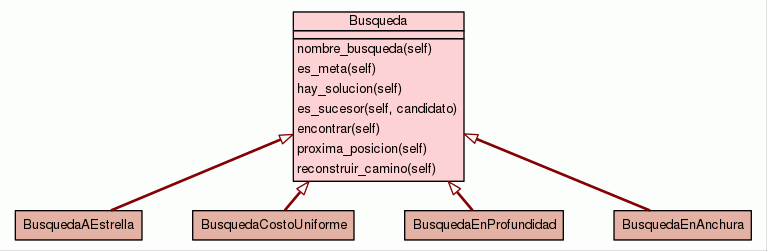
\includegraphics[scale = 0.5]{images/diagram_busq}
        \caption{Diagrama de Clases}
    \end{center}
\end{figure}

\begin{figure}[H]
    \begin{center}
        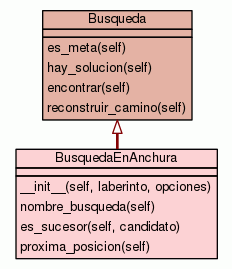
\includegraphics[scale = 0.5]{images/diagram_bea}
        \caption{Diagrama de Clases: Búsqueda en Anchura}
    \end{center}
\end{figure}

\begin{figure}[H]
    \begin{center}
        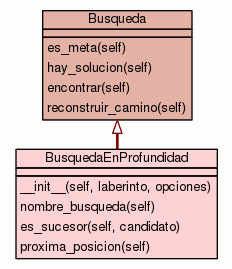
\includegraphics[scale = 0.5]{images/diagram_bep}
        \caption{Diagrama de Clases: Búsqueda en Profundidad}
    \end{center}
\end{figure}

\begin{figure}[H]
    \begin{center}
        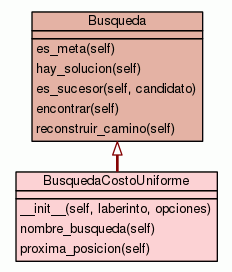
\includegraphics[scale = 0.5]{images/diagram_bcu}
        \caption{Diagrama de Clases: Búsqueda por Costo Uniforme}
    \end{center}
\end{figure}

\begin{figure}[H]
    \begin{center}
        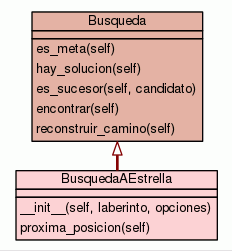
\includegraphics[scale = 0.5]{images/diagram_bae}
        \caption{Diagrama de Clases: Búsqueda A*}
    \end{center}
\end{figure}





\subsubsection{Código de la clase ``Laberinto''}
\begin{lstlisting}
    class Laberinto:
        """Esta clase representa al laberinto. Tiene como entrada un mapa en formato 
        texto el cual es procesado por esta clase y guardado en un objeto para su 
        posterior uso.
        """
        
        def __init__(self, opciones):
            """Crea una instancia de la clase Laberinto
            
            :param opciones: Valores opcionales para inicializar las variables de clase
            """
            self._opciones = opciones
    
            # Si no hay un mapa como entrada se usa el mapa de ejemplo
            if self._opciones.mapa:
                self._mapa_path = self._opciones.mapa
            else:
                self._mapa_path = self._input_path()
    
            self._mapa = self._leer_mapa()
            self._filas = len(self._mapa)
            self._columnas = len(self._mapa[0])
    
            # 3 representa a la meta
            self._posicion_meta = self.obtener_posicion(3)
    
            # 2 representa al jugador
            self._posicion_inicial_jugador = self.obtener_posicion(2)
    
        @staticmethod
        def _input_path():
            """Retorna el path del archivo laberinto usado como ejemplo"""
            pathfile = os.path.dirname(os.path.abspath(__file__))
            return os.path.join(pathfile, "..", "input", "laberinto.txt")
    
        def _leer_mapa(self):
            """Lee el mapa de entrada el cual esta en formato texto. Retorna una 
            representacion del mapa en una lista."""
            # Primero verifica si el archivo existe, sino existe crea una excepcion
            if os.path.isfile(self._mapa_path) == False:
                error_msg = "Archivo de entrada no existe: " + self._mapa_path
                raise LaberintoExcepcion(error_msg)
    
            # Lee el archivo de entrada y a la vez remueve el salto de linea al final
            lineas = [linea.strip() for linea in open(self._mapa_path)]
    
            # Transforma un caracter en una representacion numerica. Donde:
            # "#" => paredes
            # "." => caminos
            # "T" => jugador
            # "S" => salida
            mapa = []
            for i in xrange(len(lineas)):
                lista = []
                cadena = lineas[i]
    
                for j in xrange(len(cadena)):
                    if cadena[j] == "#":
                        lista.append(0)
                    elif cadena[j] == ".":
                        lista.append(1)
                    elif cadena[j] == "T":
                        lista.append(2)
                    elif cadena[j] == "S":
                        lista.append(3)
    
                mapa.append(lista)
    
            return mapa
    
        def obtener_posicion(self, objeto):
            """Retorna las coordenadas de un objecto especifico"""
            for f in xrange(self._filas):
                for c in xrange(self._columnas):
                    if self._mapa[f][c] == objeto:
                        return [f, c]
    
        def obtener_filas(self):
            """Retorna las filas"""
            return self._filas
    
        def obtener_columnas(self):
            """Retorna las columnas"""
            return self._columnas
    
        def obtener_matriz_laberinto(self):
            """Returna la representacion del mapa"""
            return self._mapa
    
        def obtener_posicion_meta(self):
            """Retorna la posicion de la meta"""
            return self._posicion_meta
    
        def obtener_posicion_inicial_jugador(self):
            """Retorna la posicion inicial del jugador"""
            return self._posicion_inicial_jugador
    
        def obtener_posiciones_libres(self, posicion_objeto):
            """Retorna las posiciones accesibles desde la posicion actual"""
            libres = []
            deltaf = [-1, 0, 1, 0]
            deltac = [0, -1, 0, 1]
            for i in xrange(4):
                nuevof = posicion_objeto[0] + deltaf[i]
                nuevoc = posicion_objeto[1] + deltac[i]
                # Se verifica que la nueva coordenada este dentro de la matriz.
                if 0 <= nuevof < self._filas and 0 <= nuevoc < self._columnas:
                    # Se verifica si es que no es una muralla ni ha sido recorrido antes.
                    if self._mapa[nuevof][nuevoc] == 1 or self._mapa[nuevof][nuevoc] == 3:
                        libres.append([nuevof, nuevoc])
    
            return libres
    
        def __str__(self):
            """Retorna el mapa en formato texto"""
            mapa_str = ""
    
            for f in xrange(self._filas):
                for c in xrange(self._columnas):
                    if self._mapa[f][c] == 0:
                        mapa_str += "# "
                    elif self._mapa[f][c] == 1:
                        mapa_str += "  "
                    elif self._mapa[f][c] == 2:
                        mapa_str += "T "
                    elif self._mapa[f][c] == 3:
                        mapa_str += "S "
                    elif self._mapa[f][c] == 4:
                        mapa_str += "* "
                    elif self._mapa[f][c] == 5:
                        mapa_str += "  "
                mapa_str += '\n'
    
            return mapa_str
\end{lstlisting}


\subsubsection{Código de la clase ``Búsqueda''}
\begin{lstlisting}
    class Busqueda:
        """Esta clase abstracta define los metodos que deben ser implementados por las 
        busquedas especificas. El fin de esta clase es estandarizar la implementacion
        de sus clases hijas.
        """
        
        def nombre_busqueda(self):
            """Retorna el tipo de busqueda."""
            raise NotImplementedError
        
        def es_meta(self):
            """Comprueba si el jugador llego a la meta."""
            return self._posicion_jugador == self._meta
    
        def hay_solucion(self):
            """Comprueba si la busqueda encontro la solucion."""
            return len(self._abiertos) != 0
    
        def es_sucesor(self, candidato):
            """Comprueba si el candidato es un sucesor."""
            raise NotImplementedError
        
        def encontrar(self):
            """Encuentra el camino."""
            while self.hay_solucion():
                if self.es_meta():
                    break
                # Si no es meta buscar otro candidato
                self.proxima_posicion()
        
        def proxima_posicion(self):
            """Encuentra los sucesores."""
            raise NotImplementedError
    
        def reconstruir_camino(self):
            """Reconstruye el camino solucion."""
            lista = list()
            #Se busca primero la posicion final (que no necesariamente es la ultima del arreglo).
            for k in xrange(len(self._camino_final)):
                if self._camino_final[k][0] == self._meta:
                    elemento = self._camino_final[k]
                    break
    
            #Se busca los padres mientras no sea el inicio.
            while elemento[1] != self._posicion_inicial:
                for i in xrange(0, len(self._camino_final)):
                    if self._camino_final[i][0] == elemento[1]:
                        elemento = self._camino_final[i]
                        lista.append(elemento[0])
                        break
            return lista
    
    
    class BusquedaEnAnchura(Busqueda):
        """Esta clase implementa busqueda en anchura."""
    
        def __init__(self, laberinto, opciones):
            """Crea una instancia de la clase BusquedaEnAnchura.
            
            :param laberinto: Es un objeto de la clase Laberinto
            :param opciones: Valores opcionales para inicializar las variables de clase
            """
    
            self._laberinto = laberinto
            self._posicion_jugador = self._laberinto.obtener_posicion_inicial_jugador()
            self._posicion_inicial = self._posicion_jugador
            self._abiertos = deque([self._posicion_jugador])
            self._meta = self._laberinto.obtener_posicion_meta()
            self._opciones = opciones
            self._camino_final = [(self._posicion_inicial, None)]
        
        def nombre_busqueda(self):
            return "Busqueda En Anchura"
        
        def es_sucesor(self, candidato):
            lista = list(self._abiertos)
            for i in xrange(len(lista)):
                if lista[i] == candidato:
                    return True
            return False
    
        def proxima_posicion(self):
            mapa = self._laberinto.obtener_matriz_laberinto()
            # Se libera la posicion actual. "4" significa "ya visitado"
            mapa[self._posicion_jugador[0]][self._posicion_jugador[1]] = 4
            self._posicion_jugador = self._abiertos.popleft()
            # Nueva posicion del jugador. "2" significa "jugador"
            mapa[self._posicion_jugador[0]][self._posicion_jugador[1]] = 2
            sucesores = self._laberinto.obtener_posiciones_libres(self._posicion_jugador)
            for sucesor in sucesores:
                if not self.es_sucesor(sucesor):
                    self._abiertos.append(sucesor)
                    self._camino_final.append((sucesor, self._posicion_jugador))
    
    
    class BusquedaEnProfundidad(Busqueda):
        """Esta clase implementa busqueda en profundidad."""
    
        def __init__(self, laberinto, opciones):
            """Crea una instancia de la clase BusquedaEnProfundidad.
            
            :param laberinto: Es un objeto de la clase Laberinto
            :param opciones: Valores opcionales para inicializar las variables de clase
            """
    
            self._laberinto = laberinto
            self._posicion_jugador = self._laberinto.obtener_posicion_inicial_jugador()
            self._posicion_inicial = self._posicion_jugador
            self._abiertos = deque([self._posicion_jugador])
            self._meta = self._laberinto.obtener_posicion_meta()
            self._opciones = opciones
            self._camino_final = [(self._posicion_inicial, None)]
        
        def nombre_busqueda(self):
            return "Busqueda En Profundidad"
        
        def es_sucesor(self, candidato):
            lista = list(self._abiertos)
            for i in xrange(len(lista)):
                if lista[i] == candidato:
                    return True
            return False
    
        def proxima_posicion(self):
            mapa = self._laberinto.obtener_matriz_laberinto()
            # Se libera la posicion actual. "4" significa "ya visitado"
            mapa[self._posicion_jugador[0]][self._posicion_jugador[1]] = 4
            self._posicion_jugador = self._abiertos.pop()
            # Nueva posicion del jugador. "2" significa "jugador"
            mapa[self._posicion_jugador[0]][self._posicion_jugador[1]] = 2
            sucesores = self._laberinto.obtener_posiciones_libres(self._posicion_jugador)
            for sucesor in sucesores:
                if not self.es_sucesor(sucesor):
                    self._abiertos.append(sucesor)
                    self._camino_final.append((sucesor, self._posicion_jugador))
    
    
    class BusquedaCostoUniforme(Busqueda):
        """Esta clase implementa busqueda de costo uniforme."""
    
        def __init__(self, laberinto, opciones):
            """Crea una instancia de la clase BusquedaCostoAnchura.
            
            :param laberinto: Es un objeto de la clase Laberinto
            :param opciones: Valores opcionales para inicializar las variables de clase
            """
    
            self._laberinto = laberinto
            self._posicion_jugador = self._laberinto.obtener_posicion_inicial_jugador()
            self._posicion_inicial = self._posicion_jugador
            self._costo_actual = 0
            self._abiertos = [(self._costo_actual, self._posicion_jugador)]
            heapify(self._abiertos)
            self._meta = self._laberinto.obtener_posicion_meta()
            self._opciones = opciones
            self._camino_final = [(self._posicion_inicial, None)]
        
        def nombre_busqueda(self):
            return "Busqueda Costo Uniforme"
        
        def proxima_posicion(self):
            mapa = self._laberinto.obtener_matriz_laberinto()
            # Se libera la posicion actual. "4" significa "ya visitado"
            mapa[self._posicion_jugador[0]][self._posicion_jugador[1]] = 4
            nodo_actual = heappop(self._abiertos)
            self._costo_actual = nodo_actual[0]
            self._posicion_jugador = nodo_actual[1]
            # Nueva posicion del jugador. "2" significa "jugador"
            mapa[self._posicion_jugador[0]][self._posicion_jugador[1]] = 2
            sucesores = self._laberinto.obtener_posiciones_libres(self._posicion_jugador)
            lista = list(self._abiertos)
            for sucesor in sucesores:
                costo = self._costo_actual + 1
                # Flag indica si es que existe o no ya en el heap el par (x,y).
                flag = False
                for i in xrange(len(lista)):
                    if lista[i][1] == sucesor:
                        flag = True
                        if lista[i][0] >= costo:
                            # Debe cambiar el costo.
                            lista[i][0] = costo
                            # Debo heapifiar.
                            heapify(lista)
                            # Esto es para reconstruir el camino.
                            for j in xrange(0, len(self._camino_final)):
                                if self._camino_final[j][0] == sucesor:
                                    self._camino_final[j] = (sucesor, self._posicion_jugador)
                # Finalmente, los que no existiesen se agregan.
                if not flag:
                    heappush(lista, [costo, sucesor])
                    # Esto es para reconstruir el camino.
                    self._camino_final.append((sucesor, self._posicion_jugador))
            #Se actualiza el heap.
            self._abiertos = lista
    
    
    class BusquedaAEstrella(Busqueda):
        """Esta clase implementa busqueda A* con una heuristica pasada por parametro."""
    
        def __init__(self, laberinto, opciones):
            """Crea una instancia de la clase BusquedaCostoAnchura.
    
            :param laberinto: Es un objeto de la clase Laberinto
            :param opciones: Valores opcionales para inicializar las variables de clase
            """
    
            self._laberinto = laberinto
            self._posicion_jugador = self._laberinto.obtener_posicion_inicial_jugador()
            self._posicion_inicial = self._posicion_jugador
            self._meta = self._laberinto.obtener_posicion_meta()
            self._costo_actual = self._funcion_heuristica(self._posicion_inicial)
            self._abiertos = [[self._costo_actual, self._posicion_jugador]]
            heapify(self._abiertos)
            self._opciones = opciones
            self._camino_final = [(self._posicion_inicial, None)]
        
        def nombre_busqueda(self):
            return "Busqueda A*"
        
        def _funcion_heuristica(self, sucesor):
            dx = abs(sucesor[0] - self._meta[0])
            dy = abs(sucesor[1] - self._meta[1])
            # Distancia de Manhattan modificada!
            return dx + dy + min(dx, dy)
    
        def proxima_posicion(self):
            mapa = self._laberinto.obtener_matriz_laberinto()
            # Se libera la posicion actual. "4" significa "ya visitado"
            mapa[self._posicion_jugador[0]][self._posicion_jugador[1]] = 4
            nodo_actual = heappop(self._abiertos)
            self._posicion_jugador = nodo_actual[1]
            self._costo_actual = nodo_actual[0] - self._funcion_heuristica(self._posicion_jugador)
            # Nueva posicion del jugador. "2" significa "jugador
            mapa[self._posicion_jugador[0]][self._posicion_jugador[1]] = 2
            sucesores = self._laberinto.obtener_posiciones_libres(self._posicion_jugador)
            lista = list(self._abiertos)
            for sucesor in sucesores:
                heuristica = self._funcion_heuristica(sucesor)
                # Flag indica si es que existe o no ya en el heap el par (x,y).
                flag = False
                for i in xrange(len(lista)):
                    if lista[i][1] == sucesor:
                        flag = True
                        if lista[i][0] >= self._costo_actual + 1 + heuristica:
                            # Debe cambiar el costo.
                            lista[i][0] = self._costo_actual + 1 + heuristica
                            # Debo heapifiar.
                            heapify(lista)
                            # Esto es para reconstruir el camino.
                            for j in xrange(0, len(self._camino_final)):
                                if self._camino_final[j][0] == sucesor:
                                    self._camino_final[j] = (sucesor, self._posicion_jugador)
                # Finalmente, los que no existiesen se agregan.
                if not flag:
                    heappush(lista, [self._costo_actual + 1 + heuristica, sucesor])
                    # Esto es para reconstruir el camino.
                    self._camino_final.append((sucesor, self._posicion_jugador))
    
            #Se actualiza el heap.
            self._abiertos = lista
\end{lstlisting}


\subsubsection{Código de la clase ``Despliegue''}
\begin{lstlisting}
    class Despliegue:
        def __init__(self, laberinto, busqueda, opciones):
            """Crea una instancia de la clase Despliegue
            
            :param laberinto: Es un objeto de la clase Laberinto
            :param busqueda: Es un objecto de la clase busqueda
            :param opciones: Valores opcionales para inicializar las variables de clase
            """
            self._laberinto = laberinto
            self._busqueda = busqueda
            self._opciones = opciones
            
            self.title = "Busqueda del Minotauro - " + self._busqueda.nombre_busqueda()
            self._width = self._laberinto.obtener_columnas() * 32
            self._height = self._laberinto.obtener_filas() * 32
    
        @staticmethod
        def _img_path():
            """Retorna el path de las imagenes"""
            pathfile = os.path.dirname(os.path.abspath(__file__))
            return os.path.join(pathfile, "..", "img")
    
        def _dibujar(self):
            """Dibuja el mapa"""
            w = 16
            h = (self._laberinto.obtener_filas() * 32 ) - 16
            mapa = self._laberinto.obtener_matriz_laberinto()
    
            img_path = self._img_path()
            grass_path = os.path.join(img_path, "grass.png")
            bloque_path = os.path.join(img_path, "bloque.png")
            ball_path = os.path.join(img_path, "ball.png")
            migas_path = os.path.join(img_path, "migas.png")
            minotauro_path = os.path.join(img_path, "minotauro.png")
    
            for f in xrange(self._laberinto.obtener_filas()):
                for c in xrange(self._laberinto.obtener_columnas()):
                    Image(grass_path, (w, h))
                    if mapa[f][c] == 0:
                        Image(bloque_path, (w, h))
                    if mapa[f][c] == 2:
                        Image(ball_path, (w, h))
                    if mapa[f][c] == 3:
                        Image(minotauro_path, (w, h))
                    if mapa[f][c] == 4:
                        Image(migas_path, (w, h))
                    w += 32
                w = 16
                h -= 32
        
        def _dibujar_solucion(self):
            """Dibuja el camino encontrado"""
            posiciones = self._busqueda.reconstruir_camino()
            camino_path = os.path.join(self._img_path(), "camino.png")
            inicio = self._laberinto.obtener_filas() * 32 - 16
            
            for p in xrange(len(posiciones)):
                h = inicio - posiciones[p][0] * 32
                w = 16 + posiciones[p][1] * 32
                Image(camino_path, (w, h))
        
        def comenzar(self):
            """Inicia el despliegue del laberinto"""
            try:
                begin_graphics(width=self._width, height=self._height, title=self.title)
                
                while self._busqueda.hay_solucion():
                    if self._busqueda.es_meta():
                        break
                    
                    # Si no es meta buscar otro candidato
                    self._busqueda.proxima_posicion()
                    
                    time.sleep(0.15)
                    clear_screen()
                    update_when('next_tick')
                    self._dibujar()
                
                if not self._opciones.auto:
                    # Se dibuja el camino recorrido solo antes de presionar una tecla
                    self._dibujar_solucion()
                    update_when('key_pressed')
            except Exception, e:
                print 'Un error ocurrio durante el dibujo: ', e
                raise
            finally:
                end_graphics()
\end{lstlisting}

\subsection{Resultados Obtenidos}
Se realizará un procedimiento estadístico ANOVA para analizar la diferencia en los tiempos medios de ejecución y el uso de memoria. Los datos en bruto se pueden observar en el apéndice C.

%----------------------------------------------------------------------------------------
% SECTION 3
%----------------------------------------------------------------------------------------
\newpage
\section{Resultados y conclusiones}
Se ha completado satisfactoriamente el objetivo del taller I que correspondía a resolver el problema del laberinto utilizando los diferentes enfoques de resolución vistos en cátedra. Este trabajo ha contribuido en el entendimiento de las técnicas de diseño de algoritmos de búsqueda no informada aprendidas mediante su implementación.

Se ha mostrado además la clara diferencia que existe en los tiempos de ejecución entre los distintos enfoques de búsquedas, como se ha comprobado con el análisis presentado.  Además se ha observado la diferencia que produce la elección de una heurística apropiada en el rendimiento del algoritmo A*.

Una observación que se debe hacer es reconsiderar el uso de la búsqueda por costo uniforme, dada la definición del costo como la cantidad de movimientos desde la posición inicial, sigue que su comportamiento es prácticamente idéntico al de búsqueda en anchura, ya que procederá a buscar por niveles. Sería diferente si existiesen diferentes tipos de suelo en el laberinto que tuviesen costos variables asociados a estos. También se debe mencionar que la búsqueda por costo uniforme es básicamente una búsqueda A* con una heurística de valor nulo,.

Se debe mencionar también el comportamiento de la búsqueda en profundidad que en algunos casos logra superar la eficiencia de A*, sin embargo, como se puede ver con uno de los laberintos en el apéndice A, el camino que encuentra no siempre es óptimo.

Un interesante problema que considerar sería agregar un elemento dinámico al ambiente, por ejemplo, un minotauro que recorriese el laberinto en busca de su víctima Teseo. Otro interesante agregado al problema, que no se realizó por falta de tiempo, sería un generador dinámico de laberintos aleatorios, con el objetivo de que las muestras utilizadas para los tiempos fueran totalmente aleatorias.

También es posible generar una extensión de los algoritmos que encuentre todas las soluciones, sin embargo, se consideró fuera del alcance de este trabajo. 

Por último queda mencionar los problemas encontrados durante el desarrollo del taller, a decir, la identificación de las posiciones ya visitadas, que correspondía a un problema del código original, y la reconstrucción de los caminos de solución, que por la estructura que tenía el código fue difícil de implementar.

%----------------------------------------------------------------------------------------
% BIBLIOGRAPHY
%----------------------------------------------------------------------------------------

\newpage
\bibliographystyle{apalike}

%Se presenta la bibliografía utilizada para el desarrollo del taller, desde los ejemplos de código utilizados, los fundamentos teóricos de los algoritmos, las herramientas para realizar el análisis de tiempo y memoria de los algoritmos y finalmente el procedimiento estadístico ANOVA.

\begin{thebibliography}{10} % 10 the total number of references
    % Libro guía
    \bibitem{Russell10} S. Russell {\em Artificial Intelligence.} 2010: A Modern Approach.
    %Heuristicas!
    \bibitem{StanfordA*} {\em Heuristics From Amit's Thoughts on Pathfinding.} Heuristics. Recuperado Junio 18, 2014, desde http://theory.stanford.edu/~amitp/GameProgramming/Heuristics.html
    
    %Experiencias
    \bibitem{1} {\em A* PathFinding Algorithm in Pacman.} Recuperado Junio 18, 2014, desde http://www.xbdev.net/maths\_of\_3d/a\_star\_pathfinding/index.php
    
    %Problema del laberinto
    \bibitem{2} {\em Buscador de Caminos con Python.} Recuperado Junio 18, 2014, desde http://razonartificial.wordpress.com/2010/01/17/buscador-de-caminos-con-python/
    
    \bibitem{3} {\em Técnicas de Inteligencia Artificial para la Solución de Laberintos de Estructura Desconocida.} Recuperado Junio 18, 2014, desde http://revistas.utp.edu.co/index.php/revistaciencia/article/viewFile/3171/1933
    
    \bibitem{4} {\em  Algoritmo de backtracking recursivo y no recursivo para la resolución de un laberinto y su aplicación en SDL.} Recuperado Junio 18, 2014, desde http://www.academia.edu/4607412/Algoritmo\_de\_Backtracking\_Recursivo\_y\_no\_Recursivo\_para\_la\_Re-solucion\_de\_un\_Laberinto\_y\_su\_Aplicacion\_en\_SDL
    
    \bibitem{5} {\em El problema del Laberinto: una versión Orientada a Objetos en Python 3.x.} Recuperado Junio 18, 2014, desde http://ic1800a2011.wordpress.com/2013/11/19/031-el-problema-del-laberinto-una-version-orientada-a-objetos-en-python-3-x/
    
    \bibitem{6} {\em Laberintos con Python.} Recuperado Junio 18, 2014, desde http://calcifer.com.ar/blog/2013/2/8/laberintos-con-python/
    
    \bibitem{7} {\em Laberinto en Python.} Recuperado Junio 18, 2014, desde http://www.solveet.com/exercises/Laberinto/185/ solution-1304

    \bibitem{8} {\em Maze Solving.} Recuperado Junio 18, 2014, desde http://rosettacode.org/wiki/Maze\_solving\#Python

    %Busqueda A*
    \bibitem{9} {\em Solving mazes using Python: Simple recursivity and A* search.} Recuperado Junio 18, 2014 desde http://www.laurentluce.com/posts/solving-mazes-using-python-simple-recursivity-and-a-search/comment-page-1/

    \bibitem{10} {\em A-star Shortest Path Algorithm (Python recipe).} Recuperado Junio 18, 2014 desde http://code.activestate.com/recipes/577519-a-star-shortest-path-algorithm/
    \bibitem{11} {\em A-Star ( A* ) search algorithm implementation.} Recuperado Junio 18, 2014 desde http://www.emoticode.net/python/a-star-a-search-algorithm-implementation.html

    %Medicion de tiempo y memoria.
    \bibitem{12} {\em A guide to analyzing Python performance.} Recuperado Junio 18, 2014 desde http://www.huyng.com/posts/python-performance-analysis/
    
    \bibitem{13} {\em Is there any simple way to benchmark python script?} Recuperado Junio 18, 2014 desde http://stackoverflow.com/questions/1593019/is-there-any-simple-way-to-benchmark-python-script


\end{thebibliography}

\newpage
\begin{appendices}
  \renewcommand\thetable{\thesection\arabic{table}}
  \renewcommand\thefigure{\thesection\arabic{figure}}
  
  \section{Imágenes de los Resultados} 
    En este anexo se presentan los resultados obtenidos por cada algoritmo en diferentes laberintos.
  
  \subsection{Búsqueda en Anchura}
  \begin{figure}[H]
  \centering
    \begin{minipage}{.5\textwidth}
        \centering
        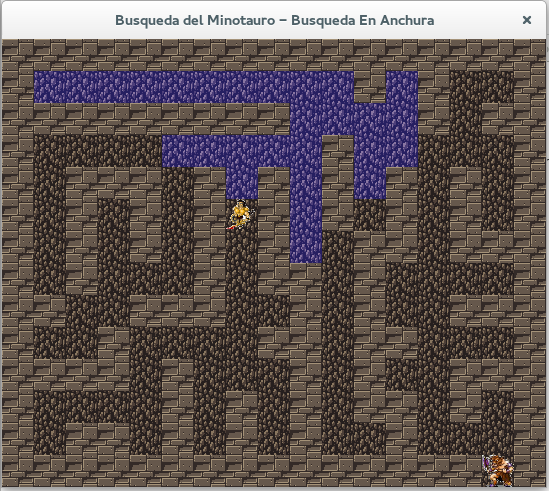
\includegraphics[width=\linewidth]{images/bea_01}
        \captionof{figure}{Búsqueda en Anchura}
    \end{minipage}%
    \begin{minipage}{.5\textwidth}
        \centering
        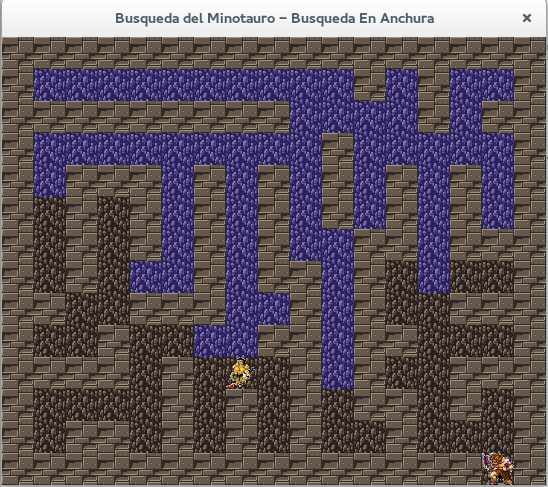
\includegraphics[width=\linewidth]{images/bea_02}
        \captionof{figure}{Búsqueda en Anchura}
    \end{minipage}
\end{figure}

\begin{figure}[H]
    \begin{center}
        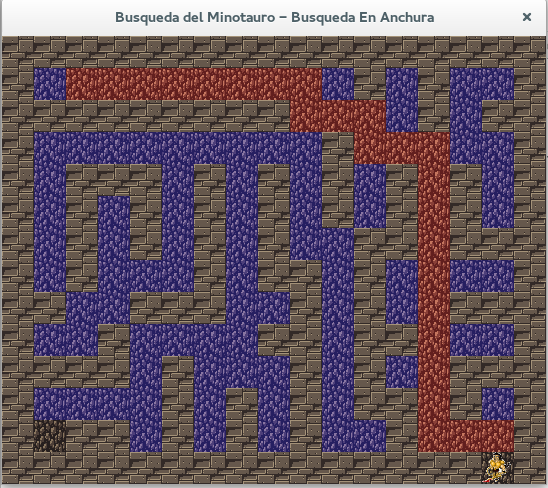
\includegraphics[scale = 0.4]{images/bea_03}
        \caption{Búsqueda en Anchura: Camino Mapa 1}
    \end{center}
\end{figure}

  
    \begin{figure}[H]
  \centering
    \begin{minipage}{.5\textwidth}
        \centering
        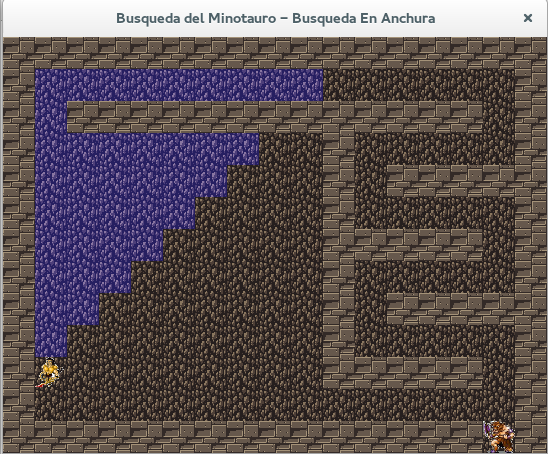
\includegraphics[width=\linewidth]{images/bea_01_m2}
        \captionof{figure}{Búsqueda en Anchura}
    \end{minipage}%
    \begin{minipage}{.5\textwidth}
        \centering
        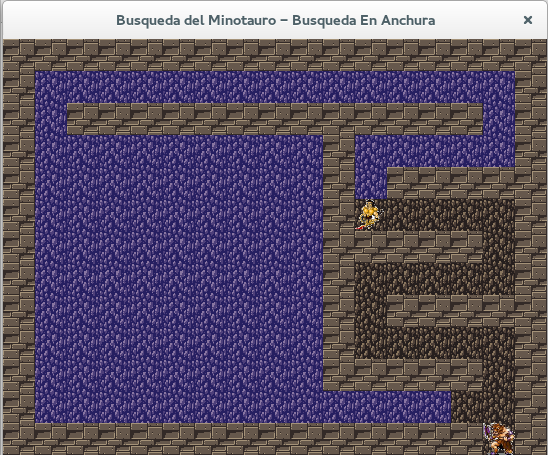
\includegraphics[width=\linewidth]{images/bea_02_m2}
        \captionof{figure}{Búsqueda en Anchura}
    \end{minipage}
\end{figure}

\begin{figure}[H]
    \begin{center}
        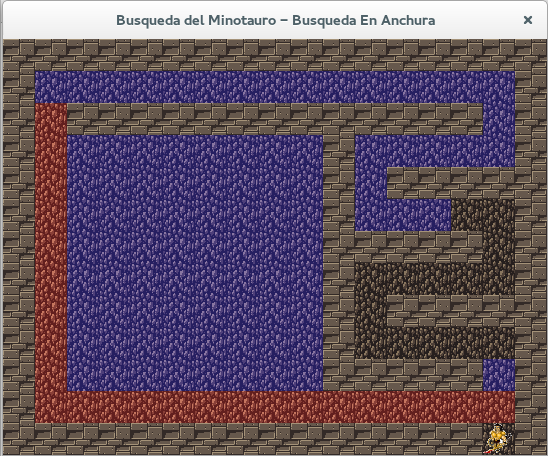
\includegraphics[scale = 0.4]{images/bea_03_m2}
        \caption{Búsqueda en Anchura: Camino Mapa 2}
    \end{center}
\end{figure}


    \begin{figure}[H]
  \centering
    \begin{minipage}{.5\textwidth}
        \centering
        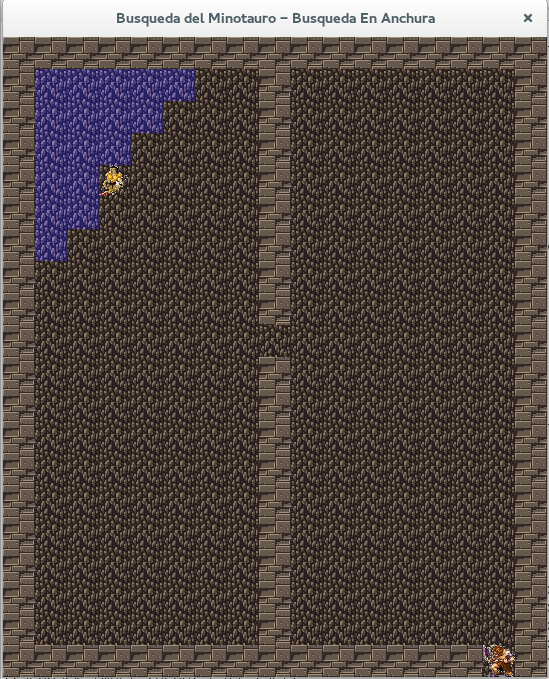
\includegraphics[width=0.8\linewidth]{images/bea_01_m3}
        \captionof{figure}{Búsqueda en Anchura}
    \end{minipage}%
    \begin{minipage}{.5\textwidth}
        \centering
        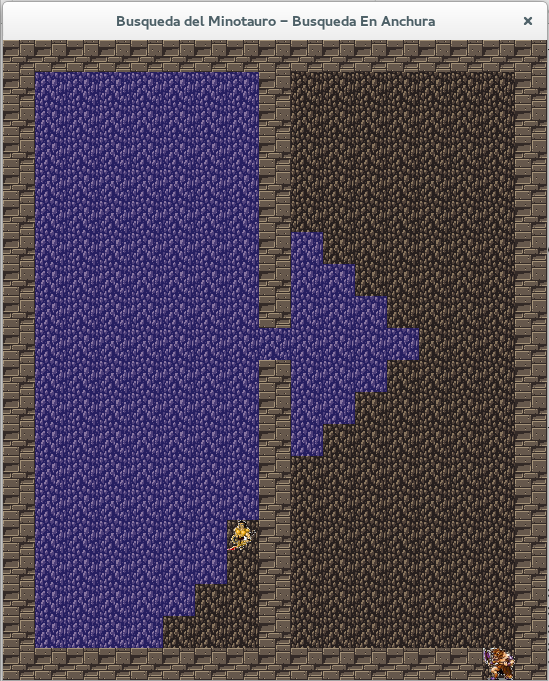
\includegraphics[width=0.8\linewidth]{images/bea_02_m3}
        \captionof{figure}{Búsqueda en Anchura}
    \end{minipage}
\end{figure}
  
  \begin{figure}[H]
    \begin{center}
        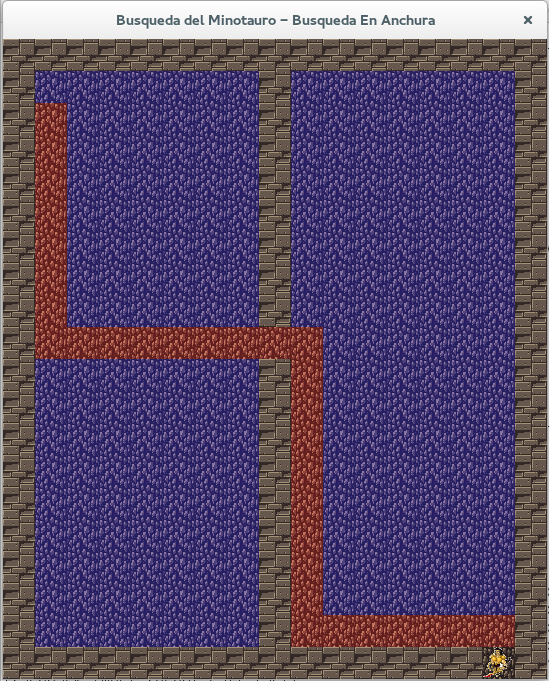
\includegraphics[scale = 0.4]{images/bea_03_m3}
        \caption{Búsqueda en Anchura: Camino Mapa 3}
    \end{center}
\end{figure}

  
  \subsection{Búsqueda en Profundidad}
  
      \begin{figure}[H]
  \centering
    \begin{minipage}{.5\textwidth}
        \centering
        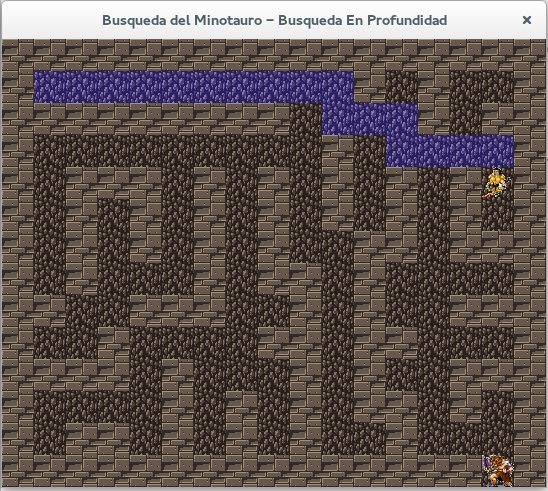
\includegraphics[width=0.8\linewidth]{images/bep_01}
        \captionof{figure}{Búsqueda en Profundidad}
    \end{minipage}%
    \begin{minipage}{.5\textwidth}
        \centering
        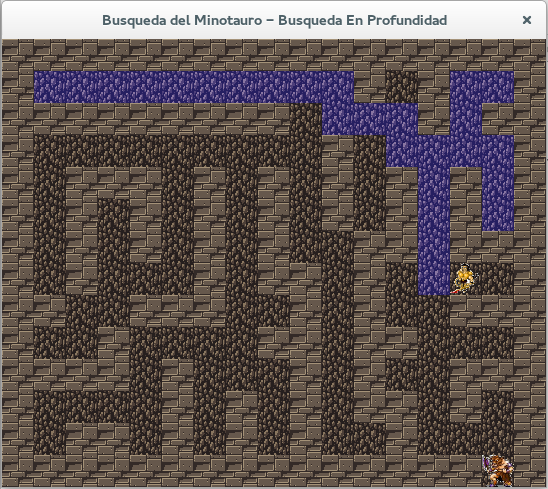
\includegraphics[width=0.8\linewidth]{images/bep_02}
        \captionof{figure}{Búsqueda en Profundidad}
    \end{minipage}
\end{figure}

  \begin{figure}[H]
    \begin{center}
        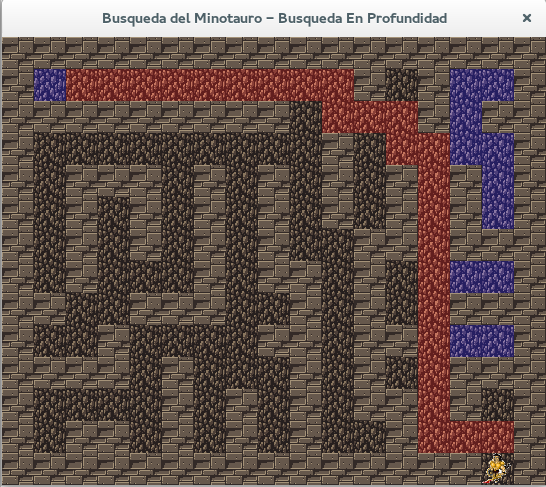
\includegraphics[scale = 0.4]{images/bep_03}
        \caption{Búsqueda en Profundidad: Camino Final}
    \end{center}
\end{figure}

  
  \subsection{Búsqueda por Costo Uniforme}
  
        \begin{figure}[H]
  \centering
    \begin{minipage}{.5\textwidth}
        \centering
        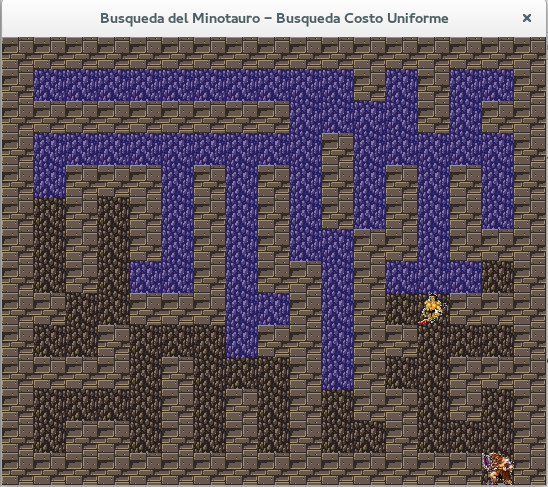
\includegraphics[width=0.8\linewidth]{images/bcu_01}
        \captionof{figure}{Búsqueda por Costo Uniforme}
    \end{minipage}%
    \begin{minipage}{.5\textwidth}
        \centering
        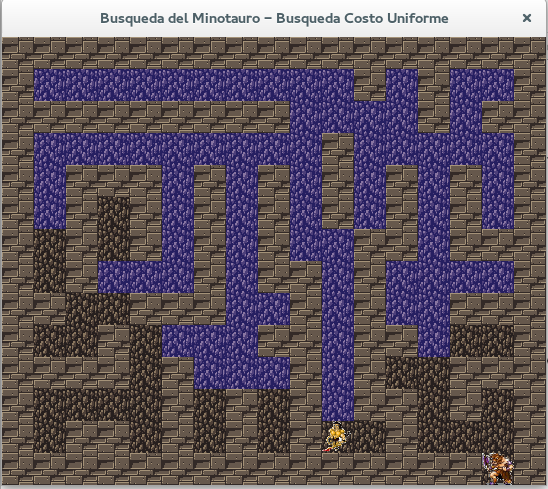
\includegraphics[width=0.8\linewidth]{images/bcu_02}
        \captionof{figure}{Búsqueda por Costo Uniforme}
    \end{minipage}
\end{figure}

  \begin{figure}[H]
    \begin{center}
        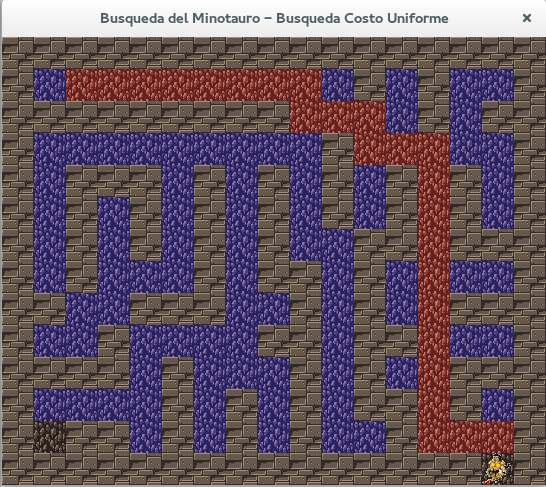
\includegraphics[scale = 0.4]{images/bcu_03}
        \caption{Búsqueda por Costo Uniforme: Camino Final}
    \end{center}
\end{figure}
  
  
  \subsection{Búsqueda A*}
    
        \begin{figure}[H]
  \centering
    \begin{minipage}{.5\textwidth}
        \centering
        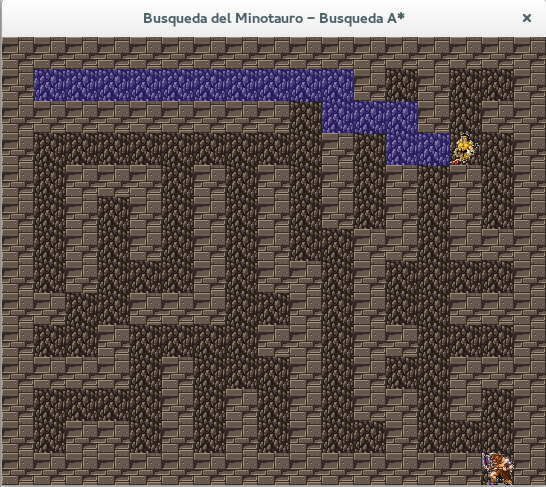
\includegraphics[width=0.8\linewidth]{images/bae_01}
        \captionof{figure}{Búsqueda A*}
    \end{minipage}%
    \begin{minipage}{.5\textwidth}
        \centering
        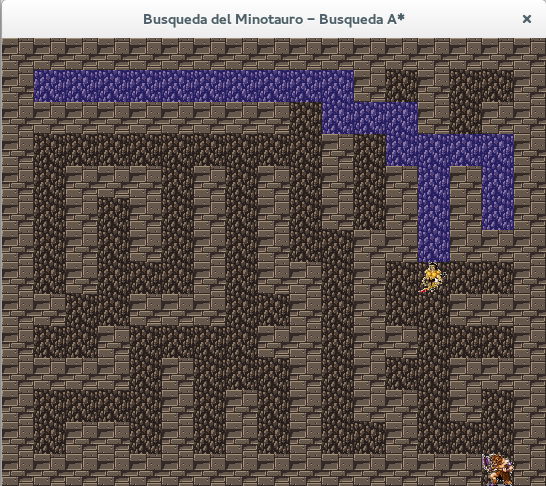
\includegraphics[width=0.8\linewidth]{images/bae_02}
        \captionof{figure}{Búsqueda A*}
    \end{minipage}
\end{figure}

  \begin{figure}[H]
    \begin{center}
        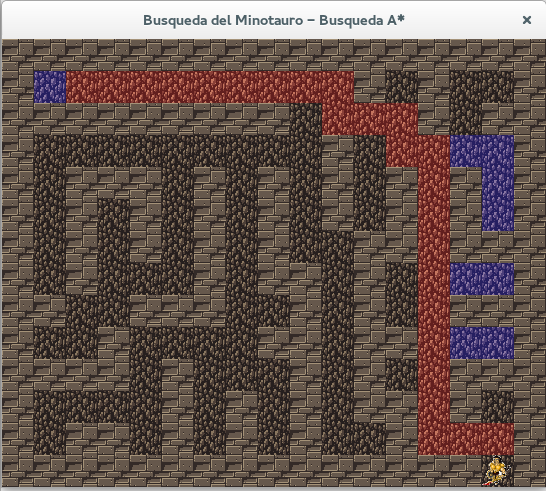
\includegraphics[scale = 0.4]{images/bae_03}
        \caption{Búsqueda A*}
    \end{center}
\end{figure}
    
    \newpage

  \section{Admisibilidad de las Heurísticas}
    En este anexo se presentan las demostraciones de admisibilidad de las heurísticas propuestas. La admisibilidad de las heurísticas garantiza la optimalidad en el algoritmo A*.
    Se debe demostrar que las heurísticas propuestas son consistentes, esto implica que es admisible, y por tanto el algoritmo A* retornará una solución óptima, se define una heurística consistente como:
\begin{align}
h(X) \leq c(X,P) + h(P)\\
h(G) = 0
\end{align}

Donde se tiene:
\begin{itemize}
\item $h$ es una función heurística consistente.
\item $N$ es cualquier nodo del grafo.
\item $P$ es cualquier sucesor de $N$.
\item $G$ es cualquier nodo objetivo.
\item $c(N,P)$ es el costo de alcanzar el nodo $P$ desde $N$.
\end{itemize}

Notar que todas las heurísticas definidas en este taller cumplen con la condición $h(G)$.

Para todas las demostraciones se definen los siguientes términos:
\begin{align}
    dx_1 = \abs{x_n-x_f}\\
  dy_1 = \abs{y_n-y_f}\\
  dx_2 = \abs{x_{n+1}-x_f}\\
  dy_2 = \abs{y_{n+1}-y_f}
\end{align}

Donde $X_n = (x_n,y_n)$, $X_{n+1} = (x_{n+1},y_{n+1})$ y $G = (x_f,y_f)$. 

\subsection{Distancia de Manhattan}

Por demostrar: $dx1 + dy1 \leq 1 + dx2 + dy2$

Cualquier movimiento realizado conserva una de las coordenadas y modifica otra, por lo tanto $dx_1 = dx_2$ o $dy_1 = dy_2$.

Sin pérdida de generalidad, asumir $dx_1 = dx_2$ (la demostración sería análoga para el otro caso):
\begin{displaymath}
  dx_1 + dy_1 = dx_2 + dy_1
\end{displaymath}

La distancia pudo aumentar, en cuyo caso:
\begin{displaymath}
dx_1 + dy_1 \leq dx_2 + dy_2 \leq 1 + dx_2 + dy_2
\end{displaymath}

La distancia pudo disminuir en a lo más una unidad, en cuyo caso:
\begin{displaymath}
dx_1 +dy_1 = dx_2 + dy_2 + 1
\end{displaymath}
Que también está cubierto por el caso $\leq$, por lo tanto la distancia de Manhattan es consistente (y por lo tanto admisible) y al utilizar la búsqueda A* con esta heurística se obtendrá una solución óptima.

\subsection{Distancia de Manhattan Modificada}
Por demostrar: $dx_1 + dy_1 + \min{(dx_1,dy_1)} \leq dx_2 + dy_2 + \min{(dx_2,dy_2)} + 2$

Cualquier movimiento conserva una de las coordenadas y modifica otro, por lo tanto se puede asumir que $dx1 = dx2$ o $dy1 = dy2$, sin pérdida de generalidad se asume que $dx_1 = dx_2$.

Luego:
\begin{displaymath}
  dx_1 + dy_1 + \min{(dx_1,dy_1)} = dx_2 + dy_1 + \min{(dx_2,dy_1)}
\end{displaymath}

Luego puede que $dy_2$ haya aumentado en 1 respecto a $dy_1$, en cuyo caso sigue que:
\begin{displaymath}
  dx_1 + dy_1 + \min{(dx_1,dy_1)} \leq dx_2 + dy_2 + \min{(dx_2,dy_2)}
\end{displaymath}


Notar que $\min{(dx_1,dy_1)} \leq \min{(dx_2,dy_2)}$, pues $dx_1 = dx_2$ y $dy_1 \leq dy_2$, en el mejor caso quedo igual, y en el peor caso aumentó en 1. 

Claramente se tiene que:
\begin{displaymath}
  dx_1 + dy_1 + \min{(dx_1,dy_1)} \leq dx_2 + dy_2 + \min{(dx_2,dy_2)} + 1
\end{displaymath}

Claramente la desigualdad se sigue cumpliendo si se suma 1 para alcanzar el valor de 2 requerido en el lado derecho.

Por otra parte, el valor del mínimo puede haber disminuido en 1, en cuyo caso:

\begin{displaymath}
  dx_1 + dy_1 + \min{(dx_1,dy_1)} = dx_2 + dy_2 + \min{(dx_2,dy_1)} + 1
\end{displaymath}

Se cambiará el lado derecho ahora por: $dx_2 + dy_2 + \min{(dx_2,dy_2)} + 1$

Notar que $\min{(dx_2,dy_2)}$ puede haber quedado igual que $\min{(dx_1,dy_1)}$ o en el peor caso haber disminuido en 1, para asegurarse que la relación es $\leq$ se debe sumar 1 al lado derecho.
\begin{displaymath}
  dx_1 + dy_1 + \min{(dx_1,dy_1)} \leq dx_2 + dy_2 + \min{(dx_2,dy_2)} + 2
\end{displaymath}
Por lo tanto la distancia de Manhattan modificada es consistente (y por lo tanto admisible) y al utilizar la búsqueda A* con esta heurística se obtendrá una solución óptima.
    
Notar que esto no se cumpliría si es que se usase un costo unitario.

\newpage
  \section{Tablas de Datos}
  En este anexo se presentan las tablas de datos referentes a los tiempos de ejecución %y uso de memoria 
  de cada uno de los algoritmos implementados.
  \subsection{Tiempo de Ejecución}

\begin{table}[H]
\begin{center}
\begin{tabular}{|l|l|l|l|l|}
\hline
\textbf{Muestra} & \textbf{BFS} & \textbf{DFS}  & \textbf{Costo Uniforme}   & \textbf{A*}   \\ \hline
1                & 0.000904     & 0.000397      & 0.001040                  & 0.000425      \\ \hline
2                & 0.000876     & 0.000346      & 0.001017                  & 0.000441      \\ \hline
3                & 0.000920     & 0.000344      & 0.001014                  & 0.000435      \\ \hline
4                & 0.000859     & 0.000457      & 0.001204                  & 0.000494      \\ \hline
5                & 0.000947     & 0.000338      & 0.001150                  & 0.000504      \\ \hline
6                & 0.001022     & 0.000341      & 0.001082                  & 0.000456      \\ \hline
7                & 0.001131     & 0.000356      & 0.001016                  & 0.000473      \\ \hline
8                & 0.000839     & 0.000332      & 0.001021                  & 0.000443      \\ \hline
9                & 0.000842     & 0.000334      & 0.001036                  & 0.000486      \\ \hline
10               & 0.000862     & 0.000348      & 0.001058                  & 0.000515      \\ \hline
\end{tabular}
\caption{Tiempos de Ejecución para cada Algoritmo.}
\end{center}
\end{table}

%  \subsection{Uso de Memoria}
%\begin{table}[H]
%\begin{center}
%\begin{tabular}{|l|l|l|l|l|}
%\hline
%\textbf{Muestra} & \textbf{BFS} & \textbf{DFS} & \textbf{Co%sto Uniforme} & \textbf{A*} \\ \hline
%1                &              &              &           %              &             \\ \hline
%2                &              &              &           %              &             \\ \hline
%3                &              &              &           %              &             \\ \hline
%4                &              &              &           %              &             \\ \hline
%5                &              &              &           %              &             \\ \hline
%6                &              &              &           %              &             \\ \hline
%7                &              &              &           %              &             \\ \hline
%8                &              &              &           %              &             \\ \hline
%9                &              &              &           %              &             \\ \hline
%10               &              &              &           %              &             \\ \hline
%\end{tabular}
%\caption{Uso de Memoria para cada Algoritmo.}
%\end{center}
%\end{table}

\end{appendices}


%----------------------------------------------------------------------------------------
%    DOCUMENT END
%----------------------------------------------------------------------------------------

\end{document}